% ============================================================
% 问题三：通信约束下的运输与中继联合调度方案
% 可直接替换模板中“问题三的模型建立与求解”部分
% ============================================================

% ---------- 问题三最终结果宏 ----------
% 若后续正式运行 q3_solver_joint_v2_1.py 后结果变化，只需修改本段宏
\newcommand{\QThreeSeed}{20260924}
\newcommand{\QThreeTransportIter}{0}
\newcommand{\QThreeJointIter}{20}

\newcommand{\QThreeBaseLate}{1131.054}
\newcommand{\QThreeBaseMakespan}{26461.112}
\newcommand{\QThreeBaseMakespanHour}{7.350}
\newcommand{\QThreeBaseEnergy}{90.744}
\newcommand{\QThreeBaseTrips}{38}

\newcommand{\QThreeLate}{752.950}
\newcommand{\QThreeMakespan}{26243.895}
\newcommand{\QThreeMakespanHour}{7.290}
\newcommand{\QThreeTransportEnergy}{83.015}
\newcommand{\QThreeRelayEnergy}{7.060}
\newcommand{\QThreeEnergy}{90.075}
\newcommand{\QThreeTransportTrips}{25}
\newcommand{\QThreeRelayTrips}{13}
\newcommand{\QThreeTrips}{38}
\newcommand{\QThreeHardViolation}{0}
\newcommand{\QThreeCommOutage}{0}
\newcommand{\QThreeScore}{0.846041}

\newcommand{\QThreeLateImprove}{33.43\%}
\newcommand{\QThreeMakespanImprove}{0.82\%}
\newcommand{\QThreeEnergyImprove}{0.74\%}
\newcommand{\QThreeScoreImprove}{15.40\%}

\section{问题三：通信约束下的运输与中继联合调度}
\label{sec:q3}

\subsection{问题分析与总体思路}

问题三在问题二异构运输无人机多点多架次调度的基础上，进一步要求运输无人机在
爬升、巡航、下降及物资投送全过程保持通信。
当运输无人机与固定网关 G01 的直连链路不可用时，
必须由空中中继无人机建立
“运输无人机--中继无人机--G01”两段链路，
并同时考虑中继悬停位置、悬停海拔、服务时段、中继实体机及能源组件周转。
因此，问题三实质上是一个同时包含
\textbf{运输路线、运输时序、通信覆盖、中继部署和双层能源资源调度}
的时空耦合优化问题。

无人机作为空中通信节点具有部署灵活、视距链路概率高等特点，
适用于地面通信基础设施受损后的临时覆盖与中继保障\cite{q3-zeng2016}；
同时，中继无人机三维位置会显著影响覆盖范围与持续服务能力，
因此悬停位置与高度不能脱离通信需求独立设置\cite{q3-mozaffari2016}。

若简单采用“先完成运输优化，再为每个运输架次配置中继”的顺序方法，
容易出现多个运输架次在不同空间盲区同时需要中继，
从而超过题目仅有的两架中继无人机容量。
为体现运输与通信的真正协同，本文构建独立的问题三求解器，
重新从原始附件读取运输、DEM、中继和通信数据，
在保持问题二统一飞行与能耗口径的同时，
将运输方案与通信保障共同纳入联合搜索。
整体求解流程为
\[
\boxed{
\begin{aligned}
&\text{原始数据读取与运输航段预计算}
\rightarrow \text{运输可行方案构造} \\
&\rightarrow \text{连续飞行轨迹离散化}
\rightarrow \text{固定网关直连判定}
\rightarrow \text{通信缺口聚类} \\
&\rightarrow \text{中继候选点搜索与双中继覆盖}
\rightarrow \text{中继资源解码} \\
&\rightarrow \text{通信冲突反馈错峰}
\rightarrow \text{通信感知 Joint-ALNS} \\
&\rightarrow \text{联合方案审计与结果输出}.
\end{aligned}}
\]

其中，问题二中使用的运输 Route Evaluator、资源解码、载荷相关能耗和共享电池周转思想
在问题三程序中独立实现，不直接调用问题二求解器或其输出文件。
这样既保证两个问题的公共物理规则一致，又允许问题三根据通信约束重新调整货箱分配和运输时序。

\subsection{运输轨迹的时空展开}

设运输架次集合为 $\mathcal{R}^{T}$。
运输架次 $r\in\mathcal{R}^{T}$ 的服务区访问序列为
\[
O01\rightarrow i_{r1}\rightarrow i_{r2}
\rightarrow\cdots\rightarrow i_{rK_r}\rightarrow O01.
\]
运输部分的容量、逐段剩余载荷、飞行时间、载荷相关能耗、返航 SOC、
硬时限和共享电池周转均沿用问题二的计算口径。
多架次无人机配送与能源约束具有典型车辆路径与资源复用特征，
相关建模思想可参见 Dorling 等关于多架次无人机配送路径与能耗约束的研究\cite{q3-dorling2017}。

为了进行通信判定，需要将每一运输架次进一步展开为随时间变化的三维轨迹。
设运输无人机在时刻 $t$ 的位置为
\begin{equation}
\mathbf{p}_r(t)
=\left(\lambda_r(t),\varphi_r(t),H_r(t)\right),
\label{eq:q3-trajectory}
\end{equation}
其中 $\lambda_r(t)$、$\varphi_r(t)$ 和 $H_r(t)$ 分别为经度、纬度和海拔。
对任一节点间航段，按照题目给定的“爬升--巡航--下降”三阶段规则进行线性时间插值；
服务区投送阶段则保持在服务区作业高度。

程序在通信规划阶段采用
\begin{equation}
\Delta t=30\ \mathrm{s}
\label{eq:q3-sample-step}
\end{equation}
的时间步长对完整飞行轨迹进行离散化，
并保留各飞行阶段端点附近的采样点。
因此，题目中的连续通信约束在数值实现中转化为对全部轨迹采样点的逐点可用性约束。

\subsection{通信链路模型}

\subsubsection{地形视距判定}

固定网关 G01 位于 O01，
其通信端点海拔由 O01 地面高程与网关天线离地高度共同确定。
对任意两个通信端点 $a,b$，
设三维位置分别为
\[
\mathbf{p}_a=(\lambda_a,\varphi_a,H_a),\qquad
\mathbf{p}_b=(\lambda_b,\varphi_b,H_b).
\]

沿两端点水平投影连线提取经过的 DEM 像元。
若某一中间 DEM 像元对应地面高程不低于两通信端点视线连线在该位置的高度，
则认为发生地形遮挡。
定义遮挡变量
\begin{equation}
\chi_{ab}=
\begin{cases}
1,&\text{端点 }a,b\text{ 之间存在地形遮挡},\\
0,&\text{否则}.
\end{cases}
\label{eq:q3-block}
\end{equation}

这种处理直接使用 30 m DEM 对山体遮挡进行判定，
从而避免仅依据二维距离估计山区通信覆盖范围。

\subsubsection{自由空间损耗与双向链路预算}

自由空间基本传播损耗按照 ITU-R P.525 建议书计算\cite{q3-itu525}。
设载波频率为 $f$ MHz，两通信端点三维距离为 $d_{ab}$ km，则
\begin{equation}
L_{ab}^{\mathrm{FS}}
=32.44+20\log_{10}f+20\log_{10}d_{ab}.
\label{eq:q3-fspl}
\end{equation}

考虑地形遮挡附加损耗 $L^{\mathrm{obs}}$ 后，
总传播损耗定义为
\begin{equation}
L_{ab}
=L_{ab}^{\mathrm{FS}}
+\chi_{ab}L^{\mathrm{obs}}.
\label{eq:q3-total-loss}
\end{equation}

设接收灵敏度为 $P^{\mathrm{sens}}$，衰落裕量为 $M^{\mathrm{fade}}$，
则有效接收门限为
\begin{equation}
P^{\mathrm{req}}
=P^{\mathrm{sens}}+M^{\mathrm{fade}}.
\label{eq:q3-receive-threshold}
\end{equation}

对于通信方向 $a\rightarrow b$，
最大允许总传播损耗为
\begin{equation}
L_{a\rightarrow b}^{\max}
=P_a^{t}+G_a^{t}+G_b^{r}
-L^{\mathrm{sys}}-P^{\mathrm{req}},
\label{eq:q3-oneway-budget}
\end{equation}
其中 $P_a^t$ 为发射功率，$G_a^t$、$G_b^r$ 分别为发射与接收天线增益，
$L^{\mathrm{sys}}$ 为系统损耗。
由于运输控制和状态回传均需可靠通信，
端点 $a,b$ 的双向链路预算取两个方向中的较小值：
\begin{equation}
L_{ab}^{\max}
=\min\left\{
L_{a\rightarrow b}^{\max},
L_{b\rightarrow a}^{\max}
\right\}.
\label{eq:q3-bidirectional-budget}
\end{equation}

因此，单链路可用变量定义为
\begin{equation}
A_{ab}(t)
=\mathbf{1}\left\{
L_{ab}(t)\le L_{ab}^{\max}
\right\}.
\label{eq:q3-link-available}
\end{equation}

\subsubsection{运输无人机通信状态}

记运输架次 $r$ 与固定网关 G01 的链路状态为
$A_{rG}(t)$，
与中继架次 $q$ 的接入链路状态为 $A_{rq}(t)$，
中继架次 $q$ 与 G01 的回传链路状态为 $A_{qG}(t)$。
若 $z_{rq}(t)=1$ 表示时刻 $t$ 由中继架次 $q$ 为运输架次 $r$ 提供保障，
则有效通信状态为
\begin{equation}
C_r(t)
=A_{rG}(t)
\vee
\left[
\bigvee_{q\in\mathcal{R}^{R}}
z_{rq}(t)A_{rq}(t)A_{qG}(t)
\right].
\label{eq:q3-communication-state}
\end{equation}

所有运输轨迹采样点均要求满足
\begin{equation}
C_r(t)=1,
\qquad r\in\mathcal{R}^{T},
\label{eq:q3-continuous-constraint}
\end{equation}
且同一运输无人机在同一时刻最多由一架中继无人机提供通信保障：
\begin{equation}
\sum_{q\in\mathcal{R}^{R}}z_{rq}(t)\le 1.
\label{eq:q3-one-relay}
\end{equation}

若 $A_{rG}(t)=0$，则将该时刻记为中继通信需求点。
程序将时间上相邻的需求点聚合成通信缺口，
从而避免为每一个离散采样点单独产生中继任务。

\subsection{中继悬停位置与中继架次模型}

\subsubsection{中继候选位置生成}

设中继候选悬停点为
\[
c=(\lambda_c,\varphi_c,H_c),
\]
其水平位置必须位于 DEM 覆盖区域内，
悬停离地高度满足
\begin{equation}
0<H_c-H_c^{\mathrm{DEM}}
\le H_R^{\max}.
\label{eq:q3-relay-height}
\end{equation}

为避免在全部 DEM 像元上进行穷举，
本文采用“通信缺口驱动的局部候选搜索”。
首先围绕失联轨迹采样点在 DEM 网格上构造候选位置，
并取若干代表性离地高度
\[
H^{\mathrm{AGL}}\in\{150,225,300\}\ \mathrm{m}.
\]
候选点首先必须满足中继--G01 回传链路可用。
随后检查其对当前通信缺口内运输轨迹采样点的覆盖情况。

对于同一时间簇，程序优先寻找一个可完整覆盖全部需求点的悬停位置；
若单点不能满足，则利用位集覆盖搜索寻找两个候选点的组合。
若粗网格下仍存在少量未覆盖采样点，
则仅在未覆盖轨迹附近加密 DEM 候选点，
避免全局细网格搜索造成过大的计算开销。
由于题目仅配置两架中继无人机，
若某一并发时间簇仍需要超过两个相互不兼容的空间中继簇，
则将该冲突反馈至运输调度层，通过错峰调整运输架次开始时刻。

\subsubsection{中继飞行与服务时间}

中继架次 $q$ 的完整任务为
\[
O01\rightarrow c_q
\rightarrow\text{悬停通信服务}
\rightarrow O01.
\]
中继从 O01 到悬停点的计划巡航海拔同样取沿线最高 DEM 高程以上 50 m。
设中继固定准备时间为 $t_R^{\mathrm{pre}}$，
飞抵悬停点所需时间为 $t_q^{\mathrm{out}}$，
建链时间为 $t_R^{\mathrm{link}}$，
通信需求开始时刻为 $s_q^{\mathrm{serv}}$，
则必须满足
\begin{equation}
s_q^{R}
+t_R^{\mathrm{pre}}
+t_q^{\mathrm{out}}
+t_R^{\mathrm{link}}
\le s_q^{\mathrm{serv}},
\label{eq:q3-relay-ready}
\end{equation}
其中 $s_q^R$ 为中继架次开始时刻。
若提前到达，中继在悬停点等待至服务开始，该等待时间同样计入悬停与通信能耗。

\subsubsection{中继能耗与返航安全约束}

设中继巡航功率、悬停功率和通信附加功率分别为
$P_R^{c}$、$P_R^{h}$ 与 $P_R^{\mathrm{com}}$，
水平单程巡航时间为 $t_q^{c}$，
往返累计爬升高度为 $h_q^{+}$，
计划起飞总质量为 $M_R$，爬升效率为 $\eta_R^{\uparrow}$。
则中继往返飞行能耗为
\begin{equation}
E_q^{\mathrm{fly}}
=
2P_R^c\frac{t_q^{c}}{3600}
+
\frac{M_Rgh_q^{+}}
{3.6\times10^6\eta_R^{\uparrow}}.
\label{eq:q3-relay-flight-energy}
\end{equation}

若服务持续时间为 $T_q^{\mathrm{serv}}$，
则建链和通信服务阶段能耗为
\begin{equation}
E_q^{\mathrm{hov}}
=
\left(P_R^h+P_R^{\mathrm{com}}\right)
\frac{t_R^{\mathrm{link}}+T_q^{\mathrm{serv}}}{3600}.
\label{eq:q3-relay-hover-energy}
\end{equation}

因此中继架次总能耗为
\begin{equation}
E_q^R
=E_q^{\mathrm{fly}}+E_q^{\mathrm{hov}}.
\label{eq:q3-relay-total-energy}
\end{equation}

若中继能源组件可用能量为 $E_R^{\mathrm{bat}}$，
返航安全余量比例为 $\rho_R$，则必须满足
\begin{equation}
E_q^R\le
(1-\rho_R)E_R^{\mathrm{bat}},
\label{eq:q3-relay-reserve}
\end{equation}
相应返航 SOC 为
\begin{equation}
SOC_q^{R}
=1-\frac{E_q^R}{E_R^{\mathrm{bat}}}
\ge \rho_R.
\label{eq:q3-relay-soc}
\end{equation}

中继能源组件的充电仍采用附件规定的两阶段等效充电模型。
同一中继无人机的两个任务区间不得重叠，
同一能源组件在“执行任务--充电--再次执行”的整个过程中不得发生资源冲突。

\subsection{通信冲突反馈与联合调度解码}

仅根据空间覆盖生成中继任务仍可能产生两类冲突：
一是同一时刻出现三个及以上相互不兼容的通信空间簇；
二是虽然空间上只需两架中继，但上一中继架次尚未返航或完成周转，
使 R01、R02 在新的通信需求开始前均不可用。

为此，程序设置外层通信联合修复机制。
当出现通信覆盖冲突时，从当前并发运输架次中优先选择时间裕量较大的架次进行错峰；
当出现中继实体机或能源组件冲突时，
根据最早可用资源时刻计算所需延迟量，并反馈至运输架次最早开始时间。
随后重新运行运输资源解码器，重新生成运输轨迹并再次规划中继。
该过程迭代至同时满足
\[
\boxed{
\text{运输资源可行}
+\text{硬时限可行}
+\text{通信覆盖可行}
+\text{中继资源可行}
}.
\]

上述反馈机制可以快速获得一份完整可行的运输--中继联合基线，
但由于其主要通过保守错峰消除冲突，
可能导致普通物资明显延迟。
因此，在可行基线之上进一步执行通信感知 Joint-ALNS。

\subsection{多目标联合优化模型}

设货箱 $b$ 的应急优先系数为 $p_b$，
实际交付完成时刻为 $T_b^{\mathrm{del}}$，
期望送达时刻为 $D_b^E$。
沿用问题二的加权迟到指标
\begin{equation}
J_L
=\sum_{b\in\mathcal B}
p_b
\frac{\max\{0,T_b^{\mathrm{del}}-D_b^E\}}
{D_b^E}.
\label{eq:q3-lateness}
\end{equation}

问题三的联合任务完成时间必须同时考虑运输无人机和中继无人机：
\begin{equation}
C_{\max}^{J}
=
\max\left\{
\max_{r\in\mathcal R^T}F_r^T,
\max_{q\in\mathcal R^R}F_q^R
\right\}.
\label{eq:q3-joint-makespan}
\end{equation}

运输与中继总能耗为
\begin{equation}
E_{\mathrm{tot}}^{J}
=\sum_{r\in\mathcal R^T}E_r^T
+\sum_{q\in\mathcal R^R}E_q^R,
\label{eq:q3-joint-energy}
\end{equation}
总架次数为
\begin{equation}
N_{\mathrm{tot}}^{J}
=|\mathcal R^T|+|\mathcal R^R|.
\label{eq:q3-joint-trips}
\end{equation}

以通信联合修复得到的完整可行基线为归一化基准，
记四项指标基准值为
$J_L^0$、$C_0^J$、$E_0^J$ 和 $N_0^J$，
构造联合目标函数
\begin{equation}
F_J
=0.45\frac{J_L}{J_L^0}
+0.25\frac{C_{\max}^{J}}{C_0^J}
+0.20\frac{E_{\mathrm{tot}}^{J}}{E_0^J}
+0.10\frac{N_{\mathrm{tot}}^{J}}{N_0^J}.
\label{eq:q3-joint-objective}
\end{equation}

其中配送及时性仍赋予最高权重，
联合完工时间次之，总能耗与两类无人机使用架次作为资源效率指标。
医疗物资及首批保障货箱硬时限、运输容量、运输返航安全余量、连续通信、中继返航安全余量及资源冲突
均作为硬约束，不参与加权折中。

\subsection{通信感知 Joint-ALNS 求解算法}

ALNS 通过多种 Destroy/Repair 算子在大邻域内重构路线，
并依据历史表现自适应调整算子使用频率，
适合求解具有容量、时间窗和多资源约束的复杂路径问题\cite{q3-ropke2006}。
针对问题三中“运输路径变化会同时改变通信需求”的特点，
本文在传统 ALNS 基础上设计通信感知结构算子，
将当前联合状态记为
\[
\mathcal S
=(\mathcal R^T,\boldsymbol{\ell},\Pi_T,\Pi_R),
\]
其中 $\mathcal R^T$ 为运输路线集合，
$\boldsymbol{\ell}$ 为各路线最早释放时刻，
$\Pi_T$ 与 $\Pi_R$ 分别表示运输和中继资源调度结果。

\subsubsection{Communication-conflict destroy}

普通随机移除无法针对中继瓶颈进行搜索。
因此，本文首先计算每一运输路线的中继占用时长
\begin{equation}
B_r
=\Delta t
\sum_{k}
\mathbf 1\{A_{rG}(t_k)=0\},
\label{eq:q3-relay-burden}
\end{equation}
并结合该路线货箱迟到贡献构造通信冲突评分
\begin{equation}
S_r^{\mathrm{des}}
=4L_r
+0.8\frac{B_r}{600}
+0.25\frac{s_r}{7200},
\label{eq:q3-destroy-score}
\end{equation}
其中 $L_r$ 为路线内普通货箱迟到贡献，$s_r$ 为路线实际开始时刻。
算法优先从高分路线中移除 1--2 个不存在硬时限的普通货箱，
并要求被破坏路线至少保留一个货箱，
以避免一次结构变化过大造成大面积不可行。

该算子的本质是优先寻找
“\textbf{送得晚且占用中继时间长}”的路线，
使后续 Repair 有机会把其中普通货箱迁移到更早、通信几何更友好的运输架次。

\subsubsection{Relay-aware repair}

对于被移除货箱 $b$，
依次尝试插入其它物理可行运输路线。
若目标路线已访问货箱所属服务区，则优先直接并入已有停靠点；
否则才尝试增加新的服务区停靠点。
这是因为同服务区回插基本不改变原运输路径的空间几何，
通常不会额外产生新的通信盲区。

对候选插入位置，构造通信感知代理代价
\begin{equation}
\begin{aligned}
C_{b\rightarrow r}^{\mathrm{rep}}
={}&\Delta C_{r}^{\mathrm{proxy}}
+0.75D_{br}
+2.2L_{br}^{\mathrm{est}} \\
&+0.15\frac{B_r}{600}
+P_{br}^{\mathrm{dir}}
-3I_{br}^{\mathrm{same}}
-0.00018\Delta T_b
+2.5I_{br}^{\mathrm{return}},
\end{aligned}
\label{eq:q3-repair-score}
\end{equation}
其中 $D_{br}$ 为新增服务区与路线已有停靠点之间的空间距离代理量，
$L_{br}^{\mathrm{est}}$ 为估计迟到代价，
$P_{br}^{\mathrm{dir}}$ 用于惩罚新增且固定网关直连条件较差的服务区，
$I_{br}^{\mathrm{same}}$ 表示目标路线是否已访问同一服务区，
$\Delta T_b$ 表示相对当前方案的提前送达量，
$I_{br}^{\mathrm{return}}$ 用于惩罚货箱重新回到原路线。
若候选插入违反硬时限，则直接排除。

对每个待修复货箱，采用 Regret 思想比较最优和次优插入位置，
优先处理“若错过当前最佳位置则后续代价显著上升”的货箱。
这样可以在改善及时性的同时尽量避免增加新的中继空间簇。

\subsubsection{时间协同邻域与接受准则}

除结构邻域外，Joint-ALNS 同时设置以下时间协同算子：

\begin{enumerate}[label=(\arabic*),leftmargin=3em]
  \item \textbf{advance-one}：尝试提前一个已被通信修复推迟的运输架次；
  \item \textbf{advance-pair}：同时提前两个运输架次，增强组合搜索能力；
  \item \textbf{reset-one}：取消一个路线的附加释放时间，重新交由资源解码器调度；
  \item \textbf{exchange-shift}：提前一个架次，同时把另一条时间裕量较大的路线适度后移，
        通过交换并发关系减轻中继资源冲突；
  \item \textbf{conflict-destroy-repair}：执行上述通信冲突 Destroy 与中继感知 Repair，直接改变货箱所属路线。
\end{enumerate}

每个候选解都必须重新运行运输资源解码、运输轨迹生成、固定网关通信判定、
中继候选搜索和中继资源解码。
只要出现硬时限违反、通信覆盖失败、中继实体机冲突或能源组件冲突，
候选解即判为不可行。

若候选联合目标优于当前解则直接接受；
对于一定程度的劣解，仍采用模拟退火概率
\begin{equation}
P_{\mathrm{acc}}
=\exp\left(-\frac{F_J^{\mathrm{new}}-F_J^{\mathrm{cur}}}{T_k}\right)
\label{eq:q3-sa}
\end{equation}
决定是否接受，其中
\begin{equation}
T_k
=\max\left\{0.004,
0.07\left(1-\frac{k}{K}\right)
\right\}.
\label{eq:q3-temperature}
\end{equation}
结构算子初始权重设为 3.2，
高于普通时间邻域，以保证有限迭代次数下能够充分搜索运输路线结构；
各算子权重根据接受及改进情况动态调整。

本文问题三程序随机种子取 \QThreeSeed，
正式计算中运输层先采用保守可行基线，
随后执行 \QThreeJointIter 次通信感知 Joint-ALNS。

\begin{table}[htbp]
  \centering
  \caption{问题三主要算法参数}
  \label{tab:q3-parameters}
  \begin{tabularx}{0.90\linewidth}{Y Y}
    \toprule
    参数 & 取值 \\
    \midrule
    通信规划时间步长 $\Delta t$ & 30 s \\
    中继候选离地高度 & 150、225、300 m \\
    单架次最大访问服务区数 & 4 \\
    运输层 ALNS 迭代次数 & \QThreeTransportIter \\
    Joint-ALNS 迭代次数 & \QThreeJointIter \\
    配送及时性权重 & 0.45 \\
    联合完工时间权重 & 0.25 \\
    运输与中继总能耗权重 & 0.20 \\
    运输与中继总架次数权重 & 0.10 \\
    Joint-ALNS 初始温度 & 0.07 \\
    Joint-ALNS 最低温度 & 0.004 \\
    随机种子 & \QThreeSeed \\
    \bottomrule
  \end{tabularx}
\end{table}
\FloatBarrier

\subsection{求解结果与分析}

\subsubsection{总体优化结果}

首先通过通信冲突反馈与中继资源解码得到完整可行基线。
该基线的加权迟到指标为 \QThreeBaseLate，
联合任务完成时间为 \QThreeBaseMakespan~s，
即约 \QThreeBaseMakespanHour~h，
运输与中继总能耗为 \QThreeBaseEnergy~kWh，
运输与中继总架次数为 \QThreeBaseTrips。

经过通信感知 Joint-ALNS 后，
最终加权迟到指标降至 \QThreeLate，
联合任务完成时间为 \QThreeMakespan~s，
即约 \QThreeMakespanHour~h；
其中运输总能耗为 \QThreeTransportEnergy~kWh，
中继总能耗为 \QThreeRelayEnergy~kWh，
合计 \QThreeEnergy~kWh。
最终共包含 \QThreeTransportTrips 个运输架次和 \QThreeRelayTrips 个中继架次，
总架次数为 \QThreeTrips，
硬时限违反数为 \QThreeHardViolation，
通信中断采样点数为 \QThreeCommOutage。

\begin{table}[htbp]
  \centering
  \caption{问题三通信联合修复基线与 Joint-ALNS 方案对比}
  \label{tab:q3-result-summary}
  \resizebox{\linewidth}{!}{
  \begin{tabular}{lccccc}
    \toprule
    方案 & 加权迟到指标 & 联合完成时间/s & 总能耗/kWh & 总架次数 & 通信中断采样点 \\
    \midrule
    通信联合修复基线
      & \QThreeBaseLate & \QThreeBaseMakespan & \QThreeBaseEnergy & \QThreeBaseTrips & 0 \\
    Joint-ALNS 方案
      & \QThreeLate & \QThreeMakespan & \QThreeEnergy & \QThreeTrips & \QThreeCommOutage \\
    \midrule
    改善幅度
      & \QThreeLateImprove & \QThreeMakespanImprove & \QThreeEnergyImprove & 0 & -- \\
    \bottomrule
  \end{tabular}}
\end{table}
\FloatBarrier

由表~\ref{tab:q3-result-summary} 可见，
Joint-ALNS 在保持运输架次和中继架次数不增加的条件下，
使加权迟到指标降低约 \QThreeLateImprove，
联合完工时间缩短约 \QThreeMakespanImprove，
总能耗下降约 \QThreeEnergyImprove。
归一化联合目标由 1.000000 降至 \QThreeScore，
总体下降约 \QThreeScoreImprove。

架次数没有继续下降并不意味着结构优化无效。
本题只有两架中继无人机，运输路线合并过度可能导致多个空间通信盲区在时间上同时出现，
反而使中继系统无法覆盖。
因此，最终算法主要通过
“\textbf{把晚期普通货箱迁移至已有同服务区的较早架次}”
改善配送及时性，
并在不增加通信空间复杂度的前提下降低后续中继负担。
这说明问题三的最优方向并非单纯追求更少运输架次，
而是需要在运输效率和通信可保障性之间进行协同权衡。

\subsubsection{运输路线与中继悬停位置}

图~\ref{fig:q3-routes-relay} 给出了最终运输路线与中继悬停位置。
图中调度中心、服务区、中继悬停点和中继部署航线分别采用不同标记，
便于观察运输路线与通信保障位置之间的空间关系。

\begin{figure}[htbp]
  \centering
  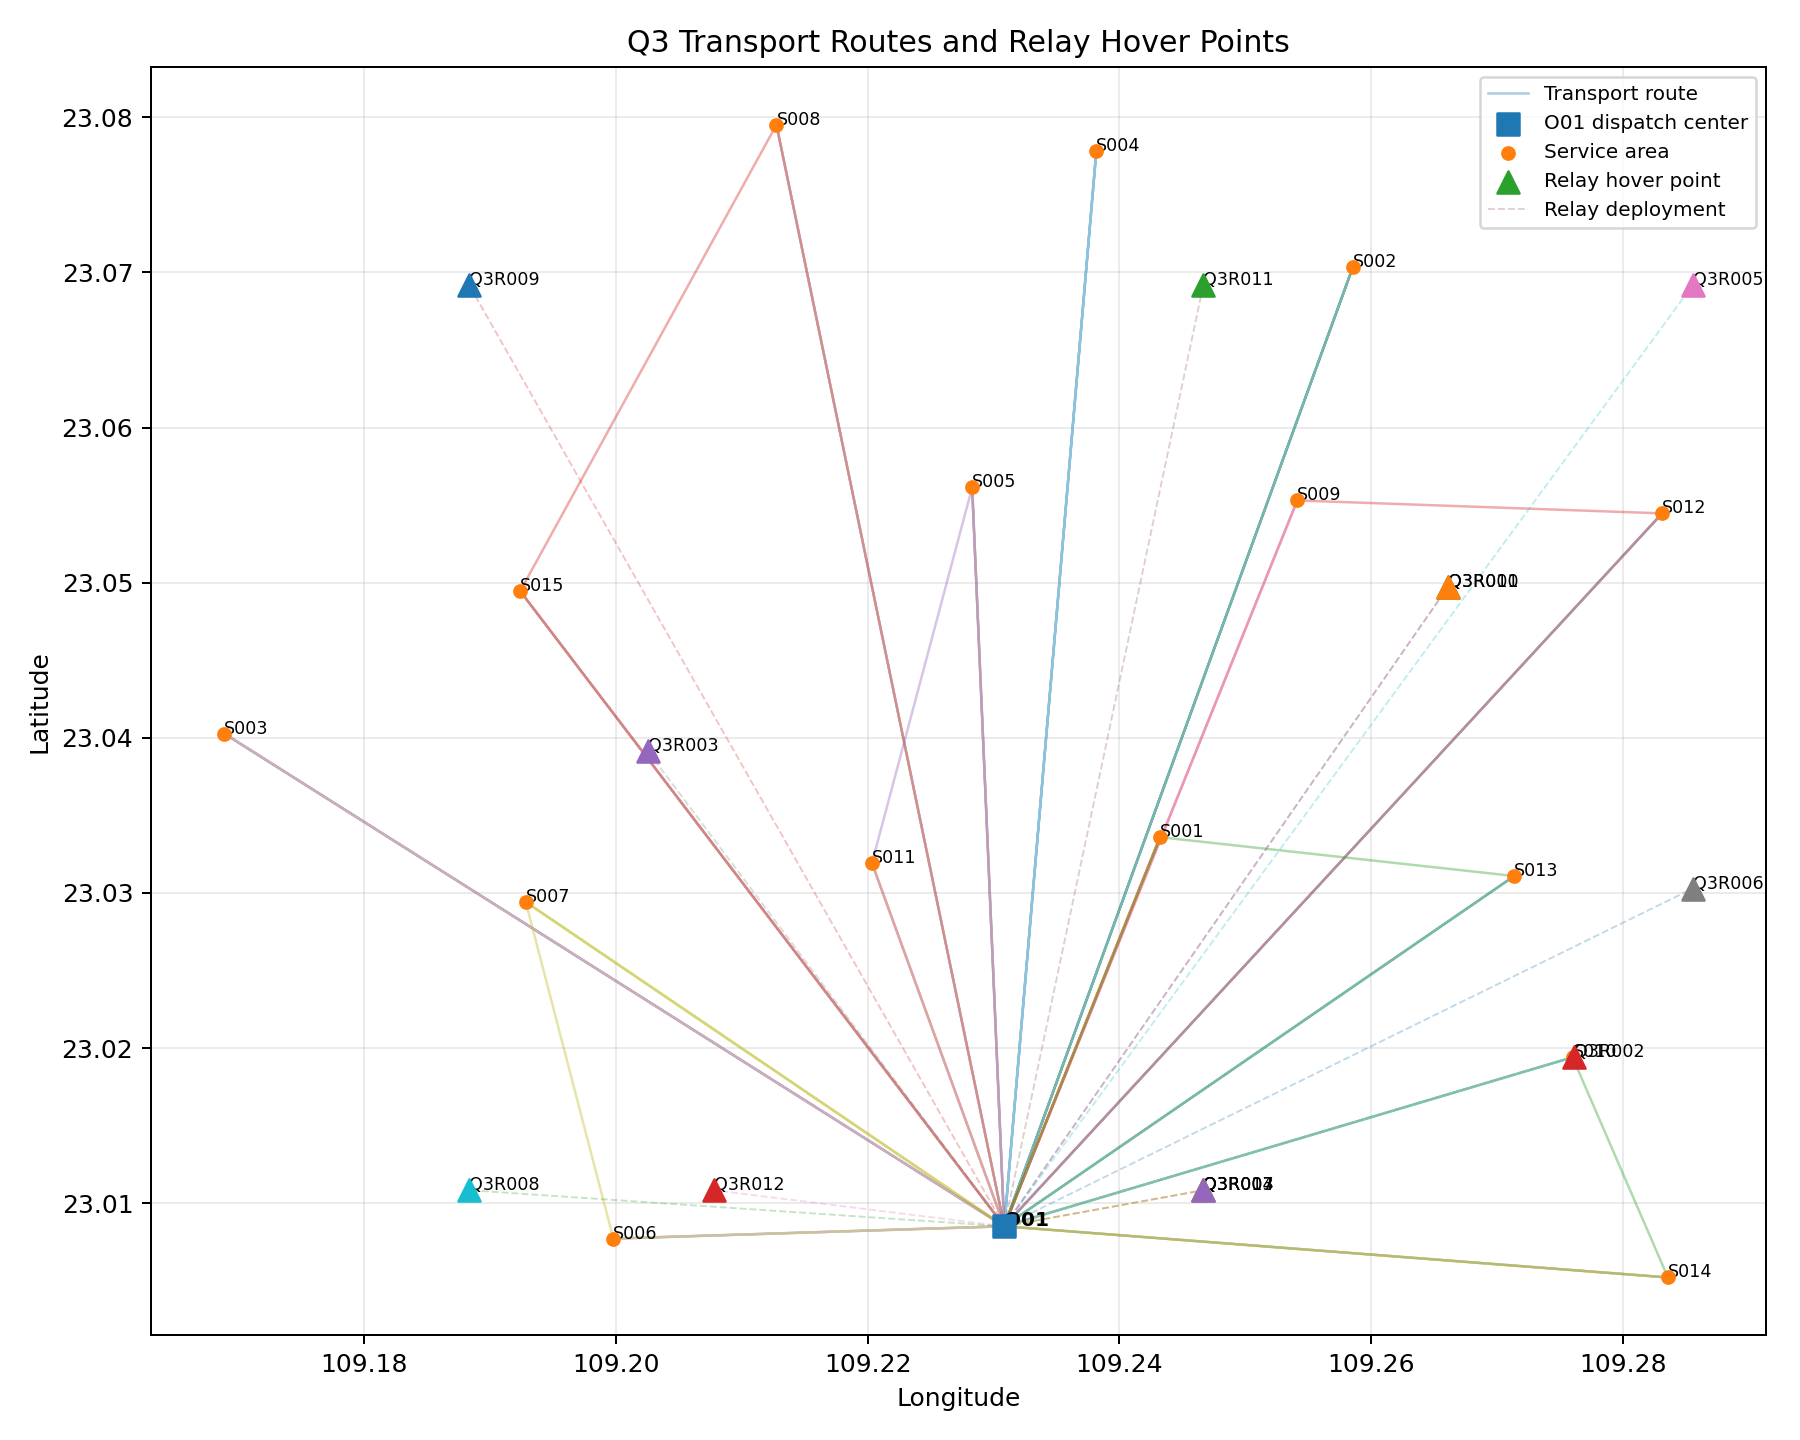
\includegraphics[width=0.95\linewidth]{../../code/3/output/fig_q3_1_routes_relay.png}
  \caption{问题三运输路线与中继悬停位置分布}
  \label{fig:q3-routes-relay}
\end{figure}
\FloatBarrier

可以看出，中继悬停点并未简单设置在服务区正上方，
而是由 DEM 地形、回传链路、运输轨迹及两架中继的联合覆盖需求共同决定。
部分悬停点可在同一服务时段覆盖多条运输轨迹，
从而避免为每个运输架次单独配置一架中继。

\subsubsection{运输--中继联合调度时序}

图~\ref{fig:q3-joint-gantt} 给出了运输无人机与中继无人机的联合调度甘特图。
运输任务与中继任务在同一时间轴上展示，
可直接观察通信需求出现前中继是否已经完成准备、飞抵和建链。

\begin{figure}[htbp]
  \centering
  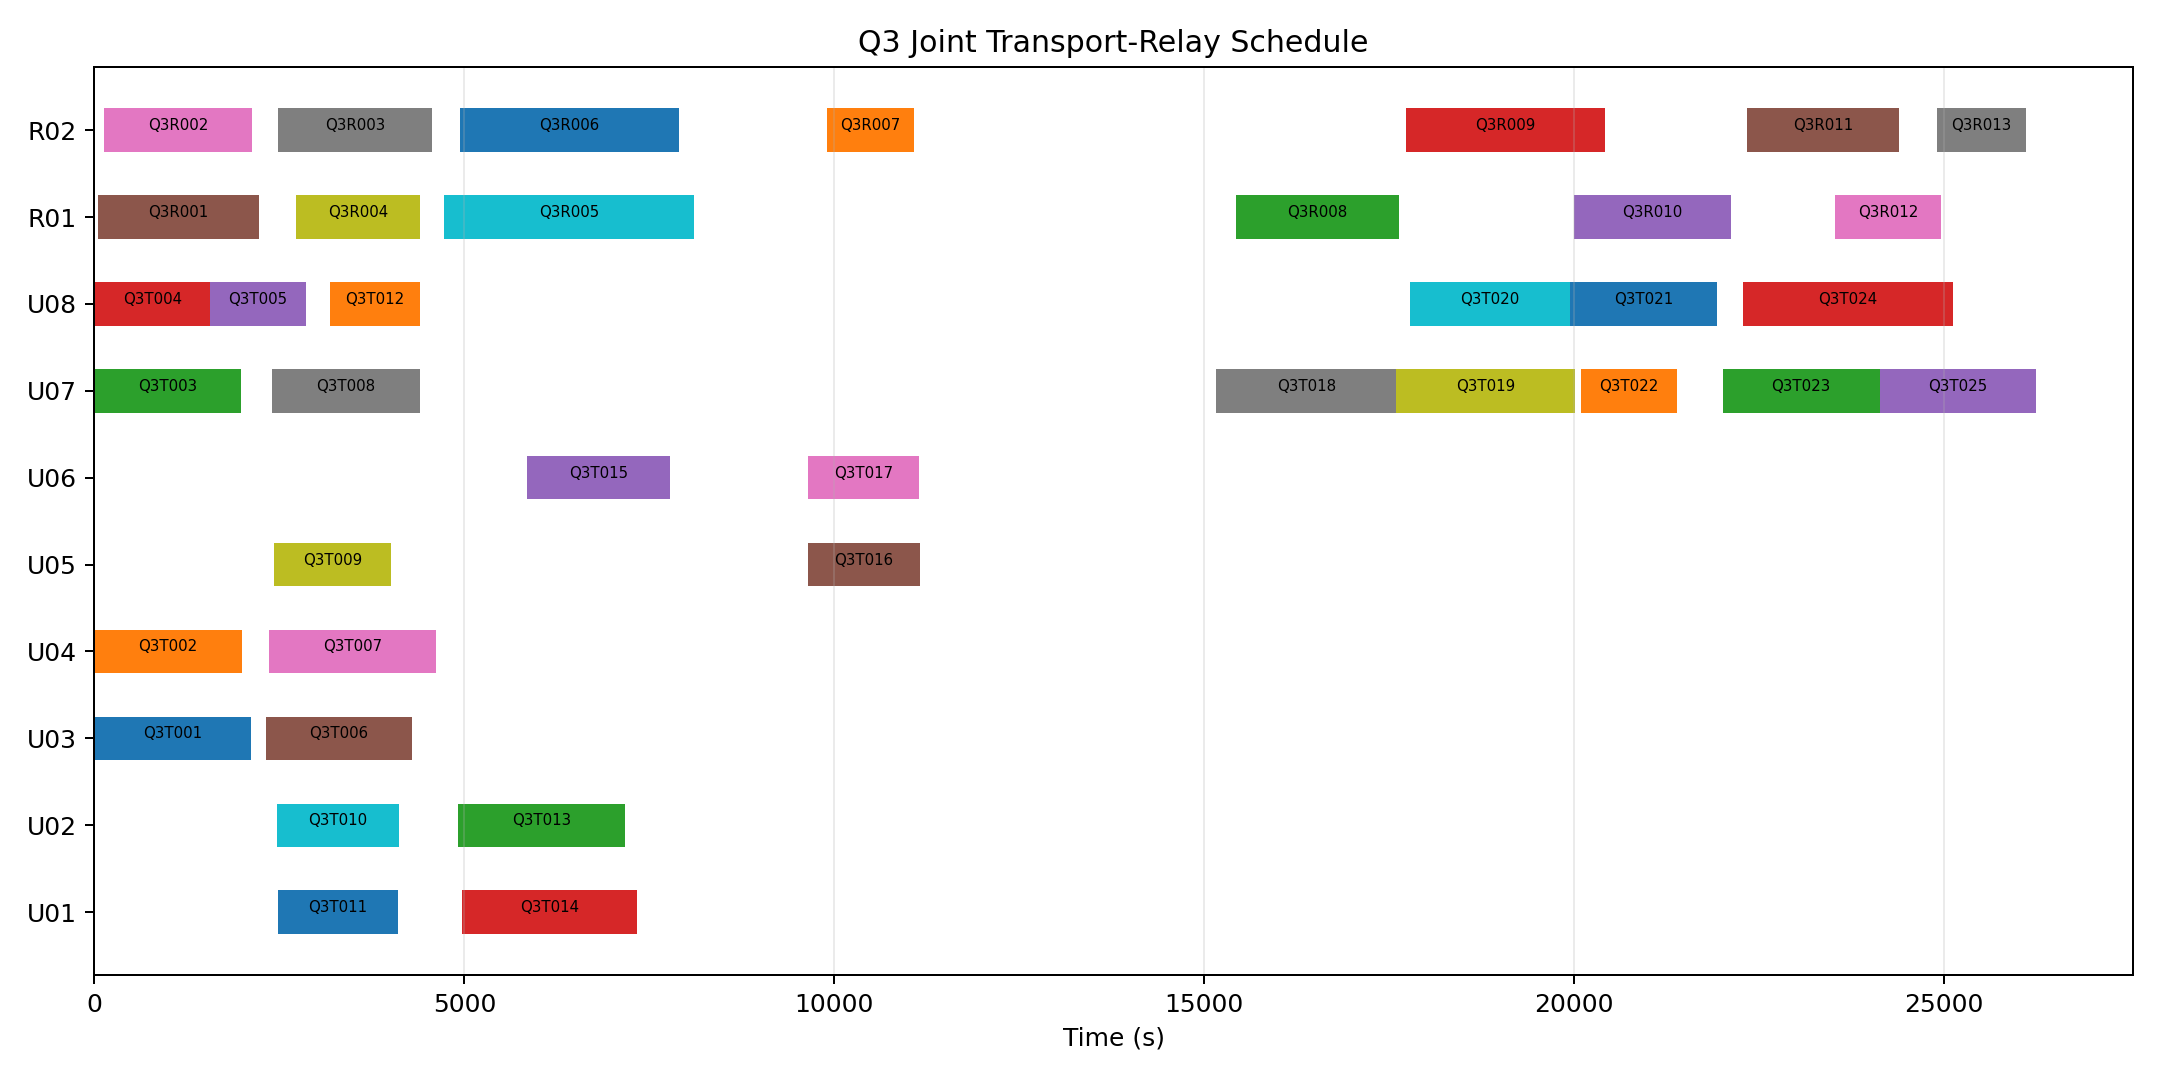
\includegraphics[width=0.96\linewidth]{../../code/3/output/fig_q3_2_joint_gantt.png}
  \caption{问题三运输无人机与中继无人机联合调度甘特图}
  \label{fig:q3-joint-gantt}
\end{figure}
\FloatBarrier

最终使用 \QThreeRelayTrips 个中继架次。
中继并非全程伴随运输无人机飞行，
而仅在固定网关直连不可用的时间段进入服务状态，
因此减少了无效悬停时间和额外通信能耗。

\subsubsection{连续通信保障状态}

图~\ref{fig:q3-comm-timeline} 按运输架次给出了固定网关直连与中继保障的时间分段。
当固定网关链路可用时优先采用直连；
进入山体遮挡或链路预算不足区间后切换至中继，
离开通信盲区后重新恢复直连。

\begin{figure}[htbp]
  \centering
  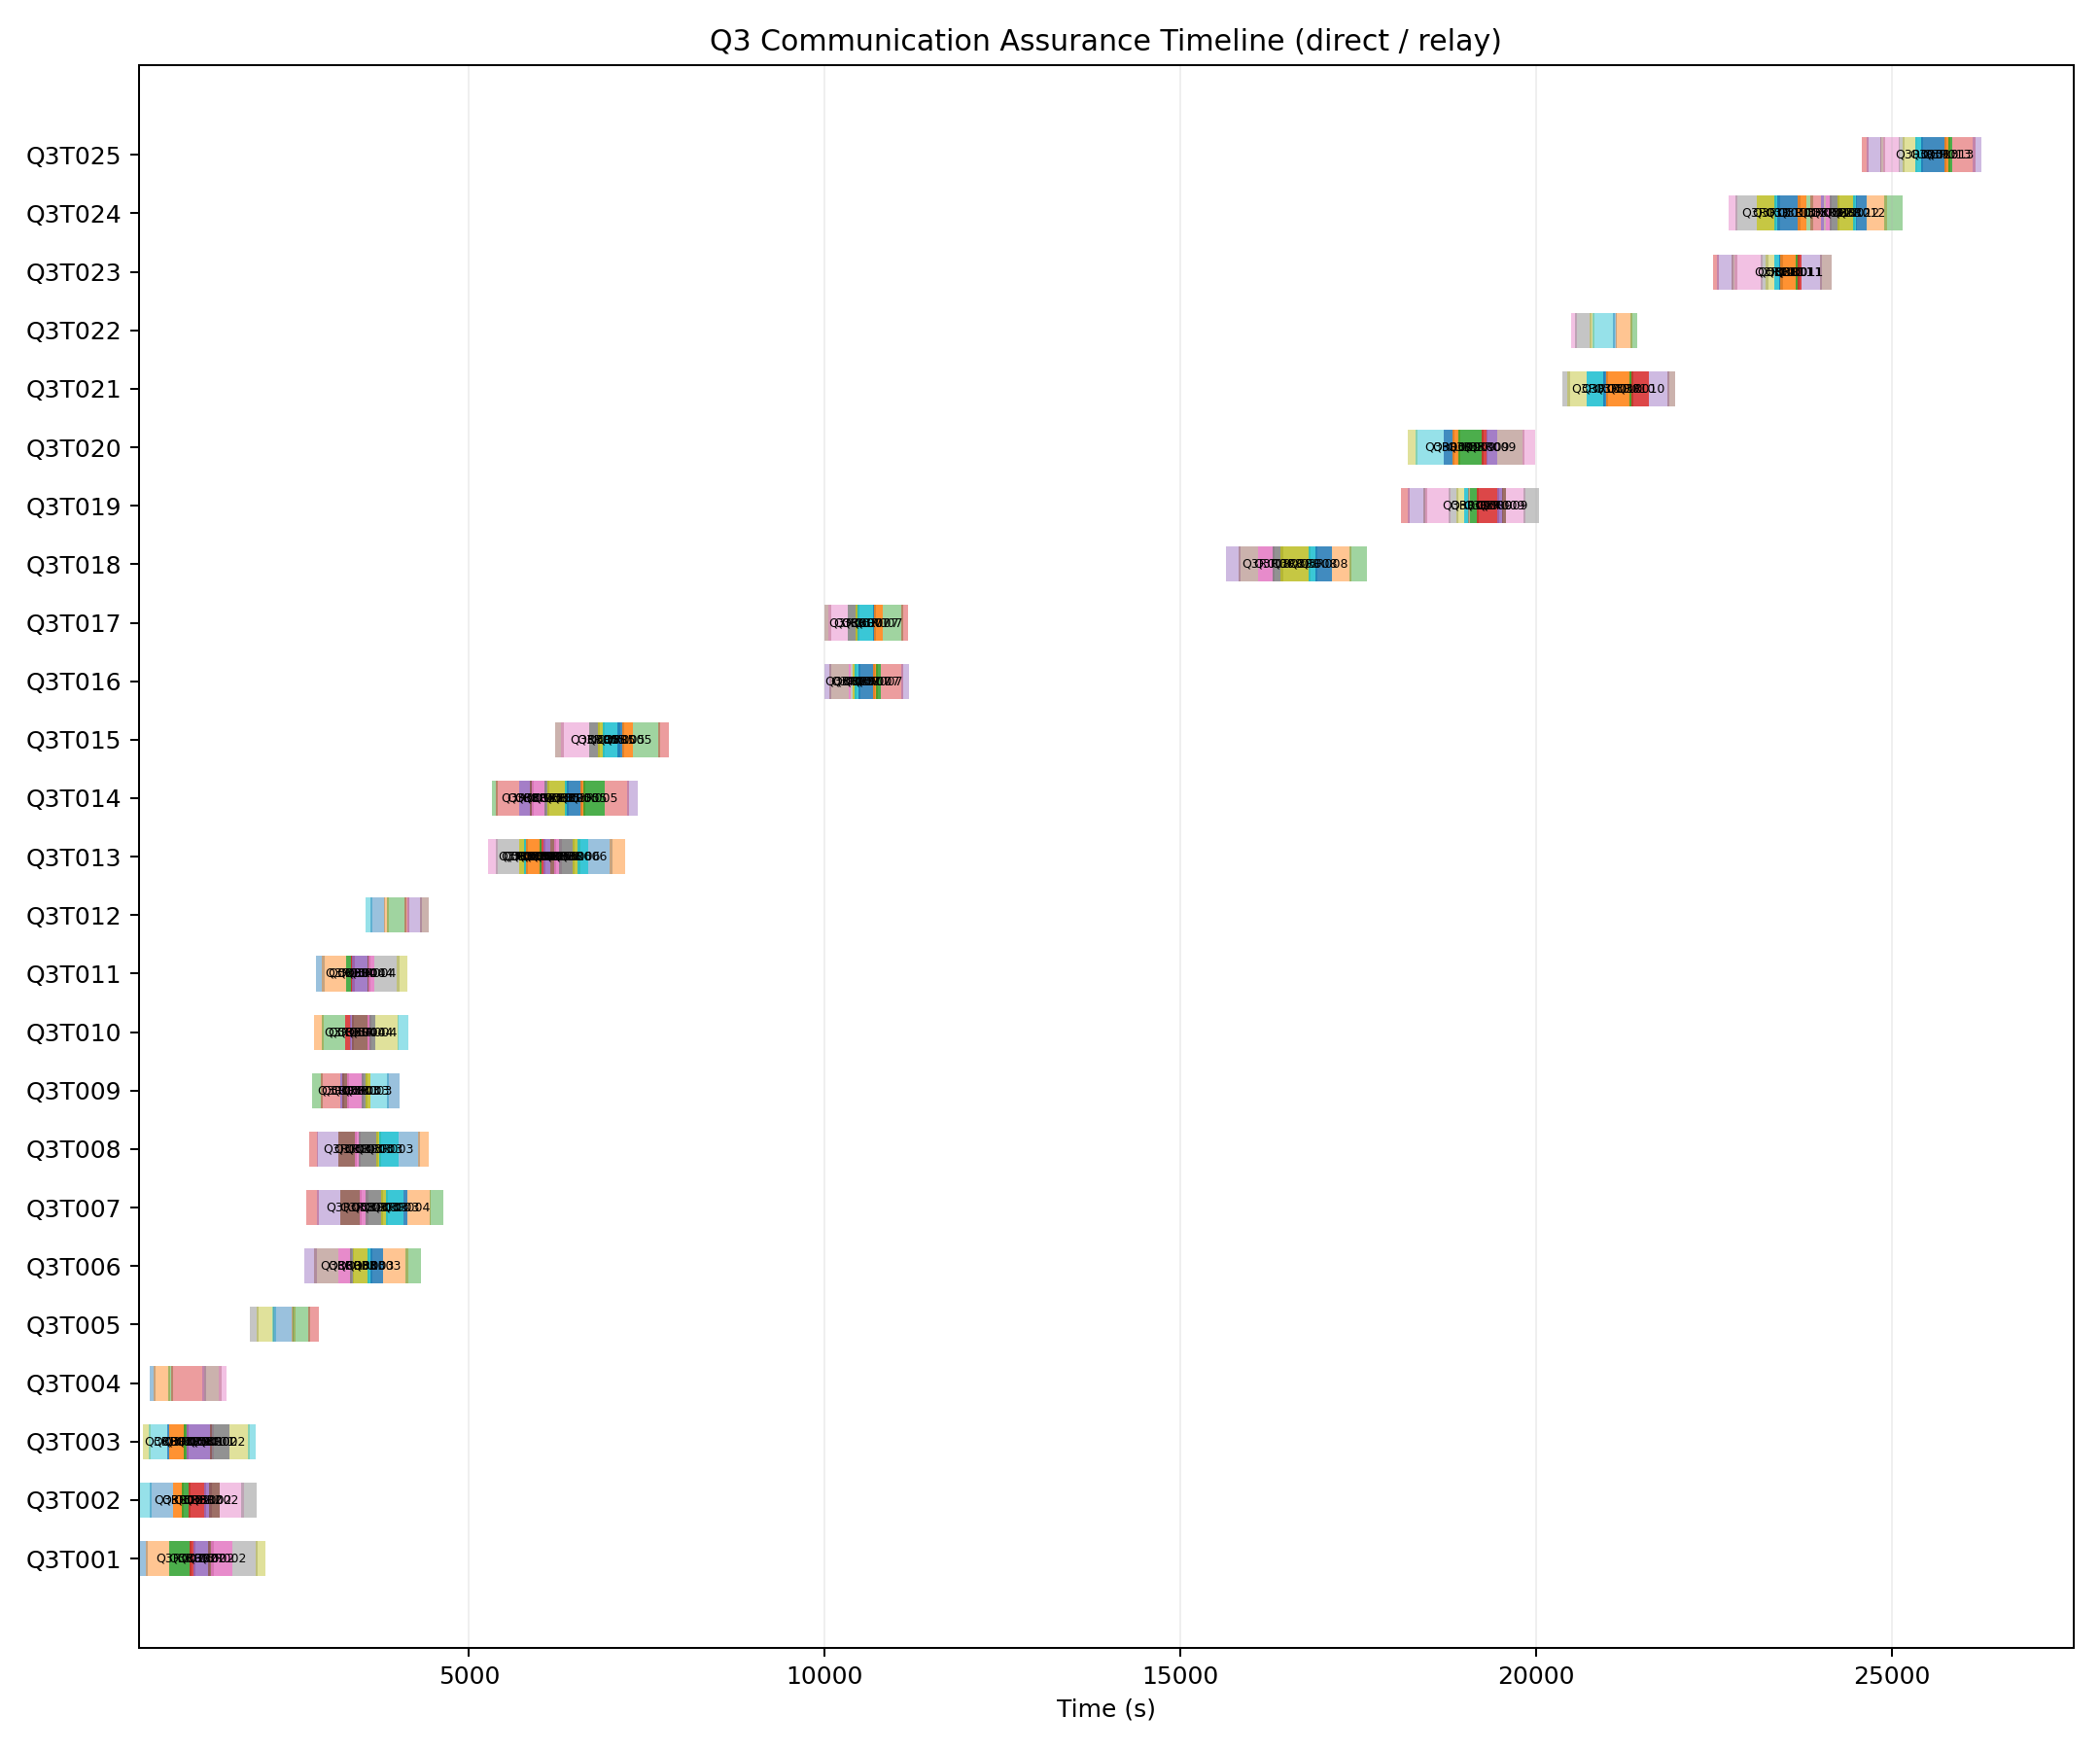
\includegraphics[width=0.97\linewidth]{../../code/3/output/fig_q3_3_comm_timeline.png}
  \caption{问题三各运输架次通信保障状态时间轴}
  \label{fig:q3-comm-timeline}
\end{figure}
\FloatBarrier

按照程序的 30 s 通信规划离散口径，
最终所有运输轨迹采样点均满足式~\eqref{eq:q3-communication-state}，
通信中断采样点数为 \QThreeCommOutage。
这表明固定网关直连与空中中继能够在整个运输任务过程中形成连续的数值覆盖链路。

\subsubsection{中继能耗与能源组件周转}

图~\ref{fig:q3-relay-energy} 给出了各中继架次能耗。
最终中继系统总能耗为 \QThreeRelayEnergy~kWh，
占运输与中继总能耗的比例较小，
说明按通信缺口部署中继比全程伴随式通信保障更加节能。

\begin{figure}[htbp]
  \centering
  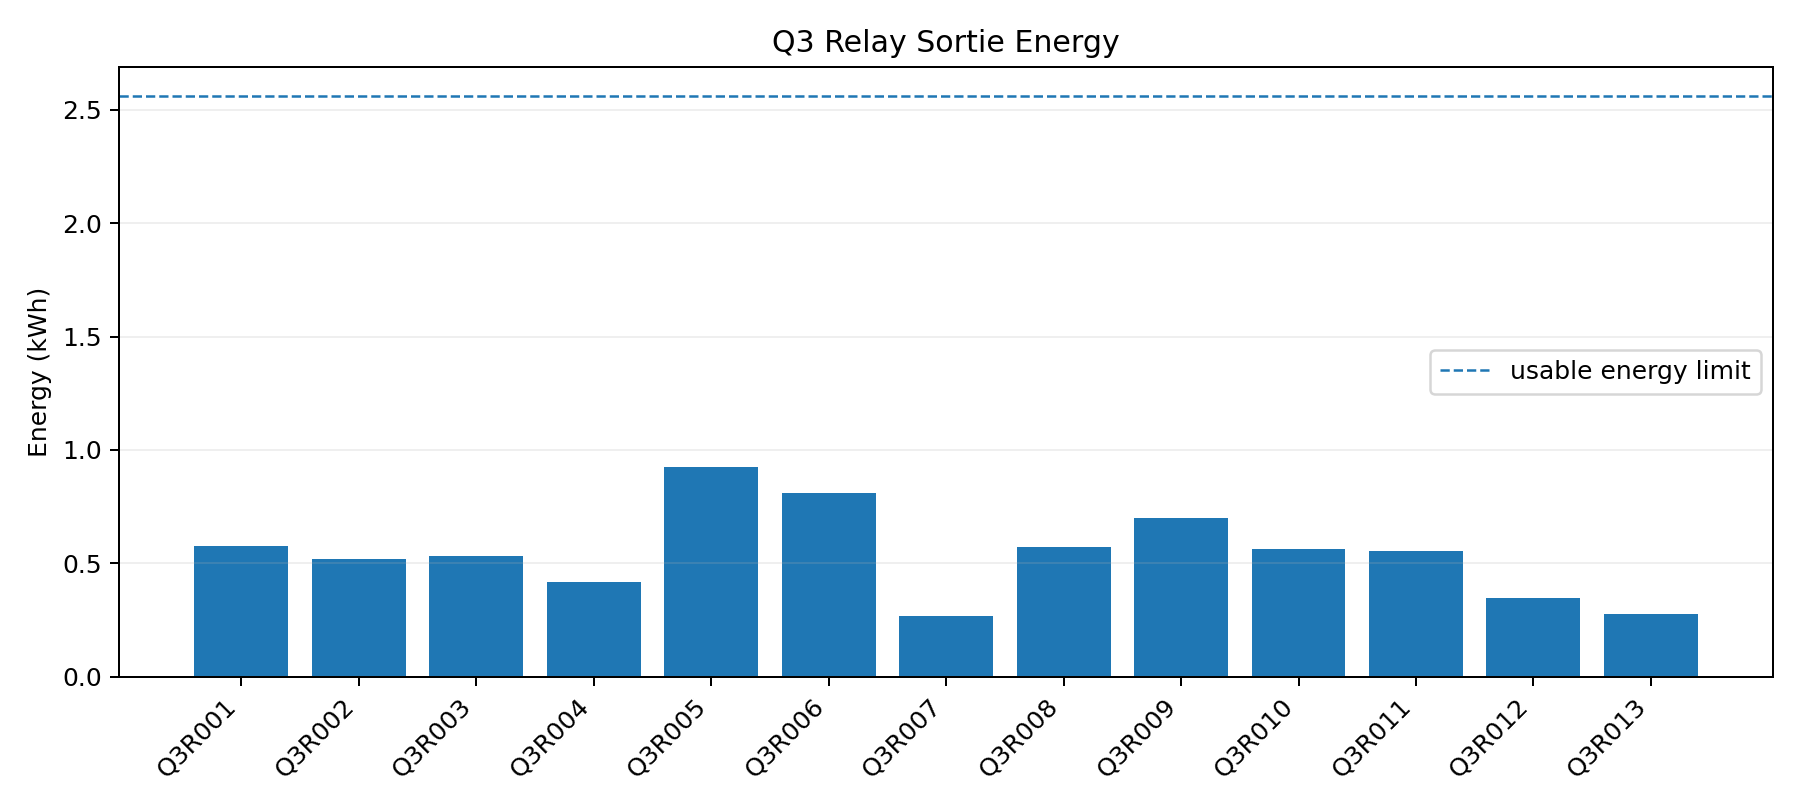
\includegraphics[width=0.90\linewidth]{../../code/3/output/fig_q3_4_relay_energy.png}
  \caption{问题三各中继架次能耗}
  \label{fig:q3-relay-energy}
\end{figure}
\FloatBarrier

所有中继架次均满足返航安全余量约束，
且 R01、R02 的任务占用时段不存在重叠；
六组能源组件按照“任务占用--返航--充电--再次可用”的顺序周转，
同一能源组件不存在并发占用。

\subsubsection{Joint-ALNS 收敛性分析}

图~\ref{fig:q3-joint-alns} 给出了通信感知 Joint-ALNS 的历史最优联合目标。
由于基线已经满足全部硬约束，初始归一化目标为 1。
结构算子开始起作用后，目标函数呈阶梯式下降，
最终稳定在 \QThreeScore。

\begin{figure}[htbp]
  \centering
  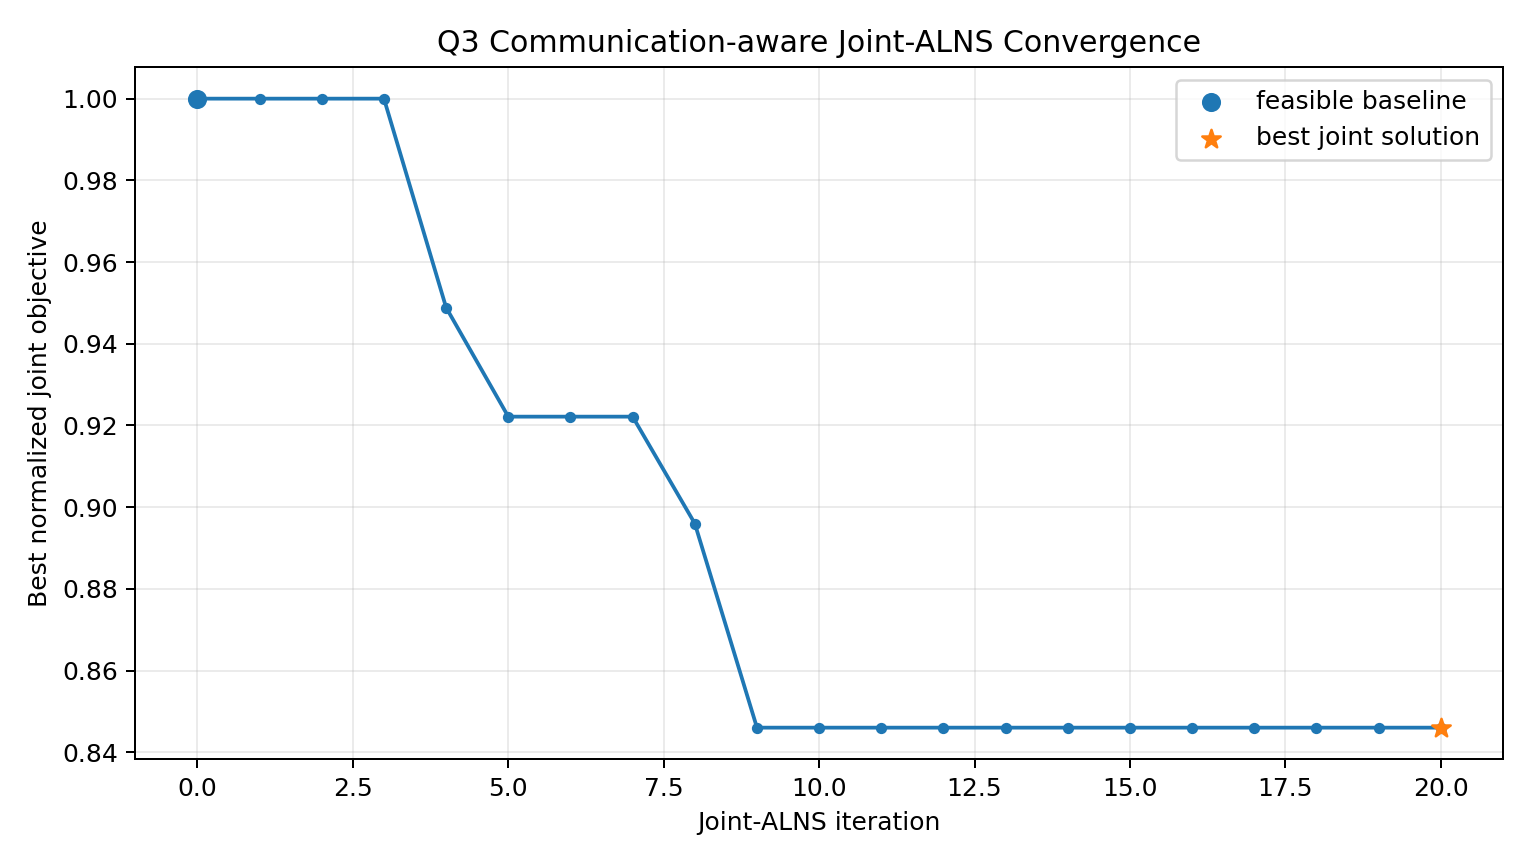
\includegraphics[width=0.82\linewidth]{../../code/3/output/fig_q3_7_joint_alns.png}
  \caption{问题三通信感知 Joint-ALNS 收敛曲线}
  \label{fig:q3-joint-alns}
\end{figure}
\FloatBarrier

搜索过程中，communication-conflict destroy 优先选取迟到贡献和中继占用均较大的路线，
relay-aware repair 则将部分普通货箱提前并入通信几何相容的早期路线。
因此，联合目标的主要改善来自配送及时性的显著提高，
同时联合完工时间和总能耗也得到小幅下降。

\subsection{方案可行性检验}

问题三比问题二多出通信链路、中继无人机和中继能源组件三类可行性条件。
为避免启发式算法产生“目标值较优但无法执行”的结果，
程序在候选状态评价和最终输出阶段均进行完整审计：

\begin{enumerate}[label=(\arabic*),leftmargin=3em]
  \item \textbf{货箱与运输路线：}
        80 个货箱均有且仅有一次交付，目的服务区正确；
  \item \textbf{运输容量与能源：}
        每个运输架次均满足载质量、体积和返航 SOC 安全余量；
  \item \textbf{配送时限：}
        医疗物资及首批保障货箱全部满足硬截止要求，
        最终硬时限违反数为 \QThreeHardViolation；
  \item \textbf{通信链路：}
        对所有运输轨迹通信采样点检查固定网关直连或中继两段链路，
        最终通信中断采样点数为 \QThreeCommOutage；
  \item \textbf{中继无人机资源：}
        同一中继无人机的架次占用时段不重叠，
        且每次均在通信需求开始前完成准备、飞抵和建链；
  \item \textbf{中继能源组件：}
        每次中继任务满足返航安全余量，
        同一能源组件的任务和充电时段不存在冲突，再次投入任务前完成充电。
\end{enumerate}

因此，最终方案满足
\[
\boxed{
\begin{aligned}
&\text{货箱唯一交付}
+\text{运输容量可行}
+\text{运输能源可行}\\
&+\text{硬时限可行}
+\text{通信保障可行}
+\text{中继能源可行}\\
&+\text{运输/中继实体资源可行}.
\end{aligned}}
\]

需要说明的是，本文采用的 Joint-ALNS 属于启发式联合优化方法，
所得结果是在当前候选点生成方式、时间离散精度、算法参数与随机种子下得到的较优可行解，
不宣称为严格意义上的全局最优解。
此外，连续通信在程序中采用 30 s 时间离散进行数值判定；
若需要进一步提高通信边界附近的验证精度，可在最终审计阶段缩小时间步长进行局部复核。

\subsection{结果文件与程序输出}

问题三程序为独立可运行文件
\texttt{q3\_solver\_joint\_v2\_1.py}，
直接读取原始节点、货箱、运输无人机、中继无人机、通信链路和 DEM 数据，
不依赖问题二求解器或问题二结果文件。

程序自动回填结果模板中的
\texttt{Q3\_中继架次} 和 \texttt{Q3\_通信保障} 两个工作表。
其中前者记录中继无人机编号、能源组件编号、开始时刻、悬停经纬度与海拔、
建链完成时刻、服务结束时刻、返航时刻及架次能耗；
后者按照通信阶段将每个运输架次的状态压缩为连续时间区间，
标记其采用“直连”或具体中继架次保障。

此外，程序输出
\texttt{Q3\_详细结果.xlsx}、
\texttt{Q3\_Joint\_ALNS日志.csv}、
中继架次与通信保障 CSV，
以及运输--中继空间分布图、联合甘特图、通信状态时间轴、
中继能耗图、通信方式占比图和 Joint-ALNS 收敛图，
从而保证论文中的主要结论与正式提交结果具有统一的数据来源和可复现性。
